\begin{applicationActivities}

\begin{activity}{5}
The image below illustrates how the linear transformation
$T : \IR^2 \rightarrow \IR^2$ given by the
standard matrix $A = \begin{bmatrix} 2 & 0 \\ 0 & 3 \end{bmatrix}$
transforms the unit square.

\begin{center}
\begin{tikzpicture}[scale=0.5]
\fill[red!50!white] (0,0) rectangle (1,1);`
\draw[thin,gray,<->] (-4,0)-- (4,0);
\draw[thin,gray,<->] (0,-4)-- (0,4);
\draw[thick,blue,->] (0,0) -- node[below] {$A \vec{e}_1= \begin{bmatrix}2 \\ 0 \end{bmatrix}$}++ (2,0);
\draw[thick,blue,->] (0,0) -- node[left] {$A \vec{e}_2 = \begin{bmatrix} 0 \\ 3 \end{bmatrix}$}++(0,3);
\draw[thick,red,->] (0,0) -- ++(1,0);
\draw[thick,red,->] (0,0) -- ++(0,1);
\draw[blue,dashed] (2,0) -- (2,3) -- (0,3);
\draw[red,dashed] (1,0) -- (1,1) -- (0,1);
\end{tikzpicture}
\end{center}

\begin{enumerate}[(a)]
\item What are the lengths of \(A\vec e_1\) and \(A\vec e_2\)?
\item What is the area of the transformed unit square?
\end{enumerate}

\end{activity}


\begin{activity}{5}
The image below illustrates how the linear transformation
$S : \IR^2 \rightarrow \IR^2$ given by the
standard matrix $B = \begin{bmatrix} 2 & 3 \\ 0 & 4 \end{bmatrix}$.
transforms the unit square.

\begin{center}
\begin{tikzpicture}[scale=0.5]
\fill[red!50!white] (0,0) rectangle (1,1);
\draw[thin,gray,<->] (-4,0)-- (4,0);
\draw[thin,gray,<->] (0,-4)-- (0,4);
\draw[thick,blue,->] (0,0) -- node[below] {$B \vec{e}_1= \begin{bmatrix}2 \\ 0 \end{bmatrix}$}++ (2,0);
\draw[thick,blue,->] (0,0) -- ++(3,4) node[above] {$B \vec{e}_2 = \begin{bmatrix} 3 \\ 4 \end{bmatrix}$};
\draw[thick,red,->] (0,0) -- ++(1,0);
\draw[thick,red,->] (0,0) -- ++(0,1);
\draw[blue,dashed] (2,0) -- (5,4) -- (3,4);
\draw[red,dashed] (1,0) -- (1,1) -- (0,1);
\end{tikzpicture}
\end{center}

\begin{enumerate}[(a)]
\item What are the lengths of \(B\vec e_1\) and \(B\vec e_2\)?
\item What is the area of the transformed unit square?
\end{enumerate}
\end{activity}

\begin{observation}
  It is possible to find two nonparallel vectors that are scaled but not rotated by
  the linear map given by \(B\).

\begin{multicols}{2}
  \[B\vec e_1=\begin{bmatrix} 2 & 3 \\ 0 & 4 \end{bmatrix}\begin{bmatrix}1\\0\end{bmatrix}
  =\begin{bmatrix}2\\0\end{bmatrix}=2\vec e_1\]

  \[
    B\begin{bmatrix}\frac{3}{4}\\\frac{1}{2}\end{bmatrix}
      =
    \begin{bmatrix} 2 & 3 \\ 0 & 4 \end{bmatrix}\begin{bmatrix}\frac{3}{4}\\\frac{1}{2}\end{bmatrix}
      =
    \begin{bmatrix}3\\2\end{bmatrix}
      =
    4\begin{bmatrix}\frac{3}{4}\\\frac{1}{2}\end{bmatrix}
  \]

\columnbreak

  \begin{center}
  \begin{tikzpicture}[scale=0.5]
  \fill[red!50!white] (0,0) -- (1,0) -- (1.75,0.5) -- (0.75,0.5) -- (0,0);
  \draw[thin,gray,<->] (-4,0)-- (4,0);
  \draw[thin,gray,<->] (0,-4)-- (0,4);
  \draw[thick,blue,->] (0,0) -- node[below] {$B\begin{bmatrix}1\\0\end{bmatrix}=2\begin{bmatrix}1\\0\end{bmatrix}$}++ (2,0);
  \draw[thick,blue,->] (0,0) -- ++(3,2) node[above] {$B\begin{bmatrix}\frac{3}{4}\\\frac{1}{2}\end{bmatrix}=4\begin{bmatrix}\frac{3}{4}\\\frac{1}{2}\end{bmatrix}$};
  \draw[thick,red,->] (0,0) -- (1,0);
  \draw[thick,red,->] (0,0) -- (0.75,0.5);
  \draw[red,dashed] (1,0) -- (1.75,0.5) -- (0.75,0.5);
  \draw[blue,dashed] (2,0) -- (5,2) -- (3,2);
  \end{tikzpicture}
  \end{center}
\end{multicols}

  The process for finding such vectors will be covered later in this module.
\end{observation}


\begin{observation}
  Notice that while a linear map can transform vectors in various ways,
  linear maps always transform parallelograms into parallelograms,
  and these areas are always transformed by the same factor: in the case of
  \(B=\begin{bmatrix} 2 & 3 \\ 0 & 4 \end{bmatrix}\),
  this factor is \(8\).
\begin{center}
\begin{tikzpicture}[scale=0.5]
\fill[red!50!white] (0,0) rectangle (1,1);
\draw[thin,gray,<->] (-4,0)-- (4,0);
\draw[thin,gray,<->] (0,-4)-- (0,4);
\draw[thick,blue,->] (0,0) -- node[below] {$B \vec{e}_1= \begin{bmatrix}2 \\ 0 \end{bmatrix}$}++ (2,0);
\draw[thick,blue,->] (0,0) -- ++(3,4) node[above] {$B \vec{e}_2 = \begin{bmatrix} 3 \\ 4 \end{bmatrix}$};
\draw[thick,red,->] (0,0) -- ++(1,0);
\draw[thick,red,->] (0,0) -- ++(0,1);
\draw[blue,dashed] (2,0) -- (5,4) -- (3,4);
\draw[red,dashed] (1,0) -- (1,1) -- (0,1);
\end{tikzpicture}
  \begin{tikzpicture}[scale=0.5]
  \fill[red!50!white] (0,0) -- (1,0) -- (1.75,0.5) -- (0.75,0.5) -- (0,0);
  \draw[thin,gray,<->] (-4,0)-- (4,0);
  \draw[thin,gray,<->] (0,-4)-- (0,4);
  \draw[thick,blue,->] (0,0) -- node[below] {$B\begin{bmatrix}1\\0\end{bmatrix}=2\begin{bmatrix}1\\0\end{bmatrix}$}++ (2,0);
  \draw[thick,blue,->] (0,0) -- ++(3,2) node[above] {$B\begin{bmatrix}\frac{3}{4}\\\frac{1}{2}\end{bmatrix}=4\begin{bmatrix}\frac{3}{4}\\\frac{1}{2}\end{bmatrix}$};
  \draw[thick,red,->] (0,0) -- (1,0);
  \draw[thick,red,->] (0,0) -- (0.75,0.5);
  \draw[red,dashed] (1,0) -- (1.75,0.5) -- (0.75,0.5);
  \draw[blue,dashed] (2,0) -- (5,2) -- (3,2);
  \end{tikzpicture}
\end{center}
Since this change in area is always the same for a given linear map,
it will be equal to the value of the transformed unit square (which
begins with area \(1\)).
\end{observation}

\begin{remark}
We will define the \term{determinant} of a square matrix \(A\),
or \(\det(A)\) for short, to be the factor by which \(A\) scales areas.  In order to figure out how to compute it, we first figure out the properties it must satisfy. 
\begin{center}
\begin{tikzpicture}[scale=0.5]
\fill[red!50!white] (0,0) rectangle (1,1);
\draw[thin,gray,<->] (-4,0)-- (4,0);
\draw[thin,gray,<->] (0,-4)-- (0,4);
\draw[thick,blue,->] (0,0) -- node[below] {$B \vec{e}_1= \begin{bmatrix}2 \\ 0 \end{bmatrix}$}++ (2,0);
\draw[thick,blue,->] (0,0) -- ++(3,4) node[above] {$B \vec{e}_2 = \begin{bmatrix} 3 \\ 4 \end{bmatrix}$};
\draw[thick,red,->] (0,0) -- ++(1,0);
\draw[thick,red,->] (0,0) -- ++(0,1);
\draw[blue,dashed] (2,0) -- (5,4) -- (3,4);
\draw[red,dashed] (1,0) -- (1,1) -- (0,1);
\end{tikzpicture}
  \begin{tikzpicture}[scale=0.5]
  \fill[red!50!white] (0,0) -- (1,0) -- (1.75,0.5) -- (0.75,0.5) -- (0,0);
  \draw[thin,gray,<->] (-4,0)-- (4,0);
  \draw[thin,gray,<->] (0,-4)-- (0,4);
  \draw[thick,blue,->] (0,0) -- node[below] {$B\begin{bmatrix}1\\0\end{bmatrix}=2\begin{bmatrix}1\\0\end{bmatrix}$}++ (2,0);
  \draw[thick,blue,->] (0,0) -- ++(3,2) node[above] {$B\begin{bmatrix}\frac{3}{4}\\\frac{1}{2}\end{bmatrix}=4\begin{bmatrix}\frac{3}{4}\\\frac{1}{2}\end{bmatrix}$};
  \draw[thick,red,->] (0,0) -- (1,0);
  \draw[thick,red,->] (0,0) -- (0.75,0.5);
  \draw[red,dashed] (1,0) -- (1.75,0.5) -- (0.75,0.5);
  \draw[blue,dashed] (2,0) -- (5,2) -- (3,2);
  \end{tikzpicture}
\end{center}
\end{remark}


\begin{activity}{2}
The transformation of the unit square by the
standard matrix \([\vec{e}_1\hspace{0.5em} \vec{e}_2]=\begin{bmatrix}1&0\\0&1\end{bmatrix}=I\) is illustrated below.
What is $\det([\vec{e}_1\hspace{0.5em} \vec{e}_2])=\det(I)$, the
area of the transformed unit square shown here?
\begin{center}
\begin{tikzpicture}[scale=1]
\fill[red!50!white] (0,0) rectangle (1,1);
\draw[thin,gray,<->] (-1,0)-- (3,0);
\draw[thin,gray,<->] (0,-1)-- (0,3);
\draw[thick,blue,->] (0,0) -- node[below] {$\vec{e}_1=\begin{bmatrix}1 \\ 0 \end{bmatrix}$} (1,0);
\draw[thick,blue,->] (0,0) -- node[left] {$\vec{e}_2=\begin{bmatrix} 0 \\ 1 \end{bmatrix}$} (0,1);
\draw[dashed,blue] (1,0) -- (1,1);
\draw[dashed,blue] (0,1) -- (1,1);
\end{tikzpicture}
\end{center}
  \begin{enumerate}[a)]
    \item 0
    \item 1
    \item 2
    \item 4
  \end{enumerate}
\end{activity}

\begin{activity}{2}
The transformation of the unit square by the
standard matrix \([\vec{v}\hspace{0.5em} \vec{v}]\) is illustrated below: both
\(T(\vec{e}_1)=T(\vect{e}_2)=\vec{v}\).
What is \(\det([\vec{v}\hspace{0.5em} \vec{v}])\), 
the area of the transformed unit square shown here?
\begin{center}
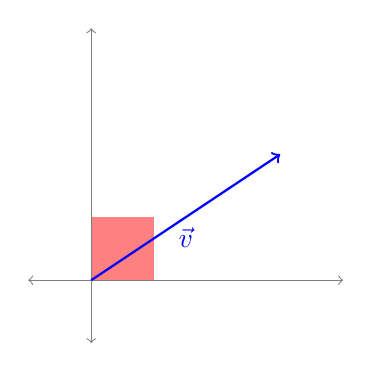
\begin{tikzpicture}[scale=0.8]
\fill[red!50!white] (0,0) rectangle (1,1);
\draw[thin,gray,<->] (-1,0)-- (4,0);
\draw[thin,gray,<->] (0,-1)-- (0,4);
\draw[thick,blue,->] (0,0) -- node[below] {$\vec{v}$} (3,2);
\end{tikzpicture}
\end{center}
  \begin{enumerate}[a)]
    \item 0
    \item 1
    \item 2
    \item 4
  \end{enumerate}
\end{activity}


\begin{activity}{5}
The transformations of the unit square by the
standard matrices \([\vec{v}\hspace{0.5em} \vec{w}]\) and
\([c\vec{v}\hspace{0.5em} \vec{w}]\) are illustrated below.
Describe the value of \(\det([c\vec{v}\hspace{0.5em} \vec{w}])\).
\begin{center}
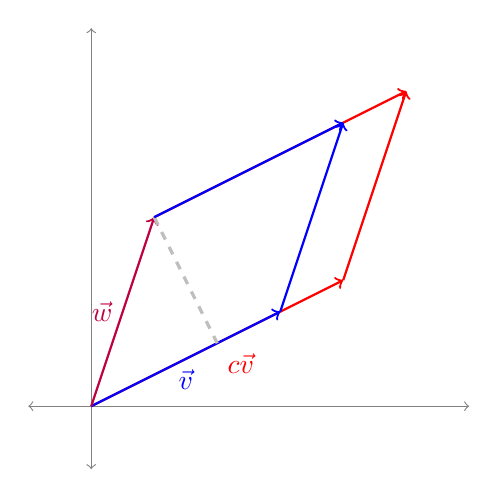
\begin{tikzpicture}[scale=0.8]
\draw[thin,gray,<->] (-1,0)-- (6,0);
\draw[thin,gray,<->] (0,-1)-- (0,6);
\draw[thick,red,->] (0,0) -- node[below right] {$c\vec{v}$}  (4,2);
\draw[thick,red,->] (1,3) -- (5,5);
\draw[thick,blue,->] (0,0) -- node[below] {$\vec{v}$} (3,1.5);
\draw[thick,purple,->] (0,0) -- node[left] {$\vec{w}$} (1,3);
\draw[lightgray,very thick,dashed] (1,3) -- (2,1);
\draw[thick,blue,->] (3,1.5) -- (4,4.5);
\draw[thick,blue,->] (1,3) -- (4,4.5);
\draw[thick,red,->] (4,2) -- (5,5);
\end{tikzpicture}
\end{center}
  \begin{enumerate}[a)]
    \item \(\det([\vec{v}\hspace{0.5em} \vec{w}])\)
    \item \(\det([\vec{v}\hspace{0.5em} \vec{w}])+c\)
    \item \(c\det([\vec{v}\hspace{0.5em} \vec{w}])\)
  \end{enumerate}
\end{activity}

\begin{activity}{5}
The transformations of unit squares by the
standard matrices \([\vec{u}\hspace{0.5em} \vec{w}]\), \([\vec{v}\hspace{0.5em} \vec{w}]\) and
\([\vec{u}+\vec{v}\hspace{0.5em} \vec{w}]\) are illustrated below.
Describe the value of \(\det([\vec{u}+\vec{v}\hspace{0.5em} \vec{w}])\).
\begin{center}
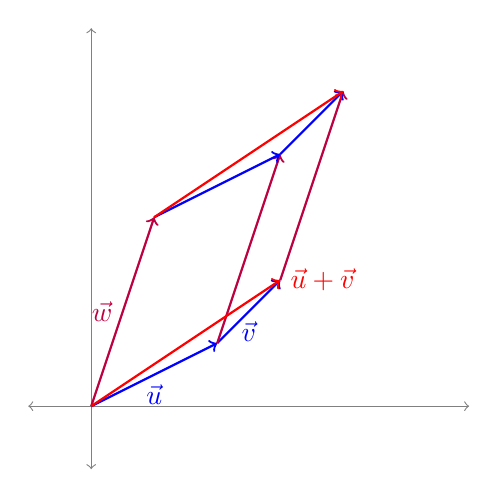
\begin{tikzpicture}[scale=0.8]
\draw[thin,gray,<->] (-1,0)-- (6,0);
\draw[thin,gray,<->] (0,-1)-- (0,6);
\draw[thick,blue,->] (0,0) -- node[below] {$\vec{u}$} (2,1);
\draw[thick,purple,->] (0,0) -- node[left] {$\vec{w}$} (1,3);
\draw[thick,blue,->] (2,1) -- node [below] {$\vec{v}$}(3,2);
\draw[thick,purple,->] (2,1) -- (3,4);
\draw[thick,purple,->] (3,2) -- (4,5);
\draw[thick,blue,->] (1,3) -- (3,4);
\draw[thick,blue,->] (3,4) -- (4,5);
\draw[thick,red,->] (0,0) --  (3,2)node[above,right] {$\vec{u}+\vec{v}$};
\draw[thick,red,->] (1,3) -- (4,5);
\end{tikzpicture}
\end{center}
  \begin{enumerate}[a)]
    \item
    \(\det([\vec{u}\hspace{0.5em} \vec{w}])=\det([\vec{v}\hspace{0.5em} \vec{w}])\)
    \item
    \(\det([\vec{u}\hspace{0.5em} \vec{w}])+\det([\vec{v}\hspace{0.5em} \vec{w}])\)
    \item
    \(\det([\vec{u}\hspace{0.5em} \vec{w}])\det([\vec{v}\hspace{0.5em} \vec{w}])\)
  \end{enumerate}
\end{activity}


\begin{definition}
The \term{determinant} is the unique function
\(\det:M_{n,n}\to\IR\) satisfying these  properties:
\begin{enumerate}
\item [P1:] $\det(I)=1$
\item [P2:] $\det(A)=0$ whenever two columns of the matrix are identical.
\item[P3:]
\(\det[\cdots\hspace{0.5em}c\vec{v}\hspace{0.5em}\cdots]=
c\det[\cdots\hspace{0.5em}\vec{v}\hspace{0.5em}\cdots]\), assuming no other columns change.
\item[P4:]
\(\det[\cdots\hspace{0.5em}\vec{v}+\vec{w}\hspace{0.5em}\cdots]=
\det[\cdots\hspace{0.5em}\vec{v}\hspace{0.5em}\cdots]+
\det[\cdots\hspace{0.5em}\vec{w}\hspace{0.5em}\cdots]\), assuming no other columns change.
\end{enumerate}

\vspace{1em}

Note that these last two properties together can be phrased as ``The determinant is linear in each column.''

\end{definition}


\begin{observation}
The determinant must also satisfy other properties.
Consider \(\det([\vec v \hspace{1em}\vec w+c \vec{v}])\) and
\(\det([\vec v\hspace{1em}\vec w])\).

\begin{center}
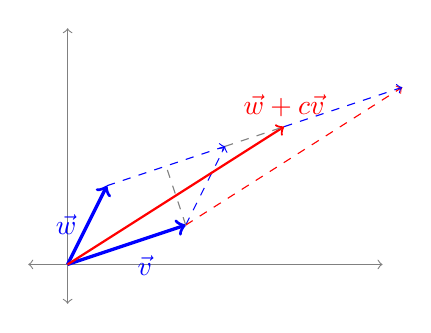
\begin{tikzpicture}[scale=0.5]
\draw[thin,gray,<->] (-1,0)-- (8,0);
\draw[thin,gray,<->] (0,-1)-- (0,6);
\draw[very thick,blue,->] (0,0) -- node[below right] {$\vec{v}$}  (3,1);
\draw[very thick,blue,->] (0,0) -- node[left] {$\vec{w}$} (1,2);
\draw[dashed,blue,->] (1,2) -- (4,3);
\draw[dashed,blue,->] (3,1) -- (4,3);
\draw[thick,red,->] (0,0) -- (5.5,3.5) node[above] {$\vec{w}+c\vec{v}$};
\draw[dashed,red,->] (3,1) -- (8.5,4.5);
\draw[dashed,blue,->] (5.5,3.5) -- (8.5,4.5);
\draw[thin,dashed,gray] (3,1) -- (2.5,2.5);
\draw[thin,dashed,gray] (4,3) -- (5.5,3.5);
\end{tikzpicture}
\end{center}

The base of both parallelograms is $\vec{v}$, while the height has not changed,
so the determinant does not change either. This can also be proven using the
other properties of the determinant:
  \begin{align*}
  \det([\vec{v}+c\vec{w}\hspace{1em}\vec{w}])
&=
  \det([\vec{v}\hspace{1em}\vec{w}])+
  \det([c\vec{w}\hspace{1em}\vec{w}])
\\ &=
  \det([\vec{v}\hspace{1em}\vec{w}])+
  c\det([\vec{w}\hspace{1em}\vec{w}])
\\ &=
  \det([\vec{v}\hspace{1em}\vec{w}])+
  c\cdot 0
\\ &=
  \det([\vec{v}\hspace{1em}\vec{w}])
  \end{align*}
\end{observation}

\begin{remark}
Swapping columns may be thought of as a reflection, which is represented by a negative
determinant. For example, the following matrices transform the unit square into
the same parallelogram, but the second matrix reflects its orientation.
\[
  A=\begin{bmatrix}2&3\\0&4\end{bmatrix}\hspace{1em}\det A=8\hspace{3em}
  B=\begin{bmatrix}3&2\\4&0\end{bmatrix}\hspace{1em}\det B=-8
\]
\begin{center}
\begin{tikzpicture}[scale=0.5]
\fill[red!50!white] (0,0) rectangle (1,1);
\draw[thin,gray,<->] (-4,0)-- (4,0);
\draw[thin,gray,<->] (0,-4)-- (0,4);
\draw[thick,blue,->] (0,0) -- node[below] {$A \vec{e}_1= \begin{bmatrix}2 \\ 0 \end{bmatrix}$}++ (2,0);
\draw[thick,blue,->] (0,0) -- ++(3,4) node[above] {$A \vec{e}_2 = \begin{bmatrix} 3 \\ 4 \end{bmatrix}$};
\draw[thick,red,->] (0,0) -- ++(1,0);
\draw[thick,red,->] (0,0) -- ++(0,1);
\draw[blue,dashed] (2,0) -- (5,4) -- (3,4);
\draw[red,dashed] (1,0) -- (1,1) -- (0,1);
\end{tikzpicture}
\begin{tikzpicture}[scale=0.5]
\fill[red!50!white] (0,0) rectangle (1,1);
\draw[thin,gray,<->] (-4,0)-- (4,0);
\draw[thin,gray,<->] (0,-4)-- (0,4);
\draw[thick,blue,->] (0,0) -- node[below] {$B \vec{e}_2= \begin{bmatrix}2 \\ 0 \end{bmatrix}$}++ (2,0);
\draw[thick,blue,->] (0,0) -- ++(3,4) node[above] {$B \vec{e}_1 = \begin{bmatrix} 3 \\ 4 \end{bmatrix}$};
\draw[thick,red,->] (0,0) -- ++(1,0);
\draw[thick,red,->] (0,0) -- ++(0,1);
\draw[blue,dashed] (2,0) -- (5,4) -- (3,4);
\draw[red,dashed] (1,0) -- (1,1) -- (0,1);
\end{tikzpicture}
\end{center}

\end{remark}


\begin{observation}
The fact that swapping columns multiplies determinants by a negative
may be verified by adding and subtracting columns.
\begin{align*}
  \det([\vec{v}\hspace{1em}\vec{w}])
&=
  \det([\vec{v}+\vec{w}\hspace{1em}\vec{w}])
\\ &=
  \det([\vec{v}+\vec{w}\hspace{1em}\vec{w}-(\vec{v}+\vec{w})])
\\ &=
  \det([\vec{v}+\vec{w}\hspace{1em}-\vec{v}])
\\ &=
  \det([\vec{v}+\vec{w}-\vec{v}\hspace{1em}-\vec{v}])
\\ &=
  \det([\vec{w}\hspace{1em}-\vec{v}])
\\ &=
  -\det([\vec{w}\hspace{1em}\vec{v}])
  \end{align*}
\end{observation}



\begin{fact}
  To summarize, we've shown that the column versions of the three row-reducing operations
  a matrix may be used to simplify a determinant in the following way:
  \begin{enumerate}[(a)]
  \item Multiplying a column by a scalar multiplies the
        determinant by that scalar:
        \[c\det([\cdots\hspace{0.5em}\vec{v}\hspace{0.5em} \cdots])=
        \det([\cdots\hspace{0.5em}c\vec{v}\hspace{0.5em} \cdots])\]
  \item Swapping two columns changes the sign of the determinant:
        \[\det([\cdots\hspace{0.5em}\vec{v}\hspace{0.5em}
        \cdots\hspace{1em}\vec{w}\hspace{0.5em} \cdots])=
        -\det([\cdots\hspace{0.5em}\vec{w}\hspace{0.5em}
        \cdots\hspace{1em}\vec{v}\hspace{0.5em} \cdots])\]
  \item Adding a multiple of a column to another column does not
        change the determinant:
        \[\det([\cdots\hspace{0.5em}\vec{v}\hspace{0.5em}
        \cdots\hspace{1em}\vec{w}\hspace{0.5em} \cdots])=
        \det([\cdots\hspace{0.5em}\vec{v}+c\vec{w}\hspace{0.5em}
        \cdots\hspace{1em}\vec{w}\hspace{0.5em} \cdots])\]
  \end{enumerate}
\end{fact}

\begin{activity}{5}
  The transformation given by the standard matrix \(A\) scales areas by
  \(4\), and the transformation given by the standard matrix \(B\) scales
  areas by \(3\). By what factor does the transformation given by the standard matrix
  \(AB\) scale areas?

\begin{center}
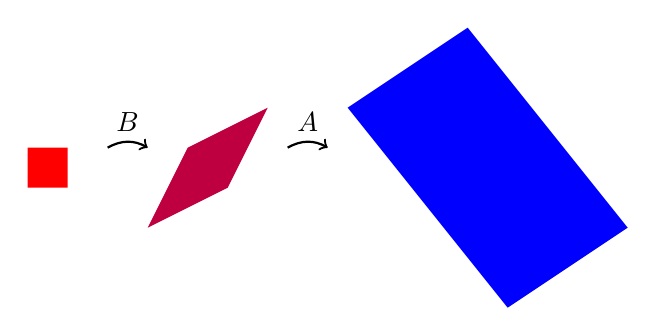
\begin{tikzpicture}[x=0.2in,y=0.2in]
\begin{scope}
\fill[red] (0,0) -- (1,0) -- (1,1) -- (0,1) -- (0,0);
\end{scope}
\draw[->,thick] (2,1) to[bend left=30] node[above] {\(B\)} (3,1);
\begin{scope}[shift={(3,-1)}]
\fill[purple] (0,0) -- (2,1) -- (3,3) -- (1,2) -- (0,0);
\end{scope}
\draw[->,thick] (6.5,1) to[bend left=30] node[above] {\(A\)} (7.5,1);
\begin{scope}[shift={(12,-3)}]
\fill[blue] (0,0) -- (-4,5) -- (-1,7) -- (3,2) -- (0,0);
\end{scope}
\end{tikzpicture}
\end{center}

  \begin{enumerate}[(a)]
  \item \(1\)
  \item \(7\)
  \item \(12\)
  \item Cannot be determined
  \end{enumerate}
\end{activity}

\begin{fact}
Since the transformation given by the standard matrix \(AB\) is obtained
by applying the transformations given by \(A\) and \(B\), it follows that 
\[\det(AB)=\det(A)\det(B)=\det(B)\det(A)=\det(BA)\]
\end{fact}

\begin{remark}
Recall that row operations may be produced by matrix multiplication.
\begin{itemize}
\item Multiply the first row of \(A\) by \(c\): \(
  \begin{bmatrix}
  c & 0 & 0 \\
  0 & 1 & 0 \\
  0 & 0 & 1
  \end{bmatrix}A
\)
\item Swap the first and second row of \(A\): \(
  \begin{bmatrix}
  0 & 1 & 0 \\
  1 & 0 & 0 \\
  0 & 0 & 1
  \end{bmatrix}A
\)
\item Add \(c\) times the third row to the first row of \(A\): \(
  \begin{bmatrix}
  1 & 0 & c \\
  0 & 1 & 0 \\
  0 & 0 & 1
  \end{bmatrix}A
\)
\end{itemize}
\end{remark}


\begin{fact}
The determinants of row operation matrices may be computed
by manipulating columns to reduce each matrix to the identity:
\begin{itemize}
\item Scaling a row: \(\det
  \begin{bmatrix}
  c & 0 & 0 \\
  0 & 1 & 0 \\
  0 & 0 & 1
  \end{bmatrix}
    =
  c\det
  \begin{bmatrix}
  1 & 0 & 0 \\
  0 & 1 & 0 \\
  0 & 0 & 1
  \end{bmatrix}
    =
  c
\)
\item Swapping rows: \(\det
  \begin{bmatrix}
  0 & 1 & 0 \\
  1 & 0 & 0 \\
  0 & 0 & 1
  \end{bmatrix}
    =
  -1\det
  \begin{bmatrix}
  1 & 0 & 0 \\
  0 & 1 & 0 \\
  0 & 0 & 1
  \end{bmatrix}
    =
  -1
\)
\item Adding a row multiple to another row: \(\det
  \begin{bmatrix}
  1 & 0 & c \\
  0 & 1 & 0 \\
  0 & 0 & 1
  \end{bmatrix}
    =
  \det
  \begin{bmatrix}
  1 & 0 & c-1c \\
  0 & 1 & 0-0c \\
  0 & 0 & 1-0c
  \end{bmatrix}
    =
  \det(I)=1
\)
\end{itemize}
\end{fact}

\begin{activity}{5}
Consider the row operation \(R_1+4R_3\to R_1\) applied as follows to show
\(A\sim B\):
\[
A=\begin{bmatrix}1&2&3\\4&5&6\\7&8&9\end{bmatrix}
  \sim
\begin{bmatrix}1+4(7)&2+4(8)&3+4(9)\\4&5&6\\7&8&9\end{bmatrix}=B
\]
\begin{enumerate}[(a)]
\item Find a matrix \(R\) such that \(B=RA\), by applying the same row operation to 
\(I=\begin{bmatrix}1&0&0\\0&1&0\\0&0&1\end{bmatrix}\).
\item Find \(\det R\) by comparing with the previous slide.
\item If \(C \in M_{3,3}\) is a matrix with \(\det(C)= -3\), find 
\[\det(RC)=\det(R)\det(C).\]
\end{enumerate}
\end{activity}

\begin{activity}{5}
Consider the row operation \(R_1\leftrightarrow R_3\) applied as follows to show
\(A\sim B\):
\[
A=\begin{bmatrix}1&2&3\\4&5&6\\7&8&9\end{bmatrix}
  \sim
\begin{bmatrix}7&8&9\\4&5&6\\1&2&3\end{bmatrix}=B
\]
\begin{enumerate}[(a)]
\item Find a matrix \(R\) such that \(B=RA\), by applying the same row operation to \(I\).
\item If \(C \in M_{3,3}\) is a matrix with \(\det(C)= 5\), find \(\det(RC)\).
\end{enumerate}
\end{activity}

\begin{activity}{5}
Consider the row operation \(3R_2\to R_2\) applied as follows to show
\(A\sim B\):
\[
A=\begin{bmatrix}1&2&3\\4&5&6\\7&8&9\end{bmatrix}
  \sim
\begin{bmatrix}1&2&3\\3(4)&3(5)&3(6)\\7&8&9\end{bmatrix}=B
\]
\begin{enumerate}[(a)]
\item Find a matrix \(R\) such that \(B=RA\).
\item If \(C \in M_{3,3}\) is a matrix with \(\det(C)= -7\), find \(\det(RC)\).
\end{enumerate}
\end{activity}


\end{applicationActivities}
